\section{Results and discussion}

\subsection{Benchmarks and verification} \label{sec:res_benchmarks}

\subsubsection{Benchmarks for the brute force approach, no repulsion or jastrow factor} \label{sec:res_N2N6_norep}
Table \ref{tab:N2_norep} shows the results from the brute force simulation of the two electron - no repulsion case. 
A plot of the results is shown in figure \ref{fig:N2_norep}. 

\begin{table}[h!]
	\centering 
	\begin{tabular}{l @{ } l @{ } l @{ } l @{ } l @{ } l @{ } l @{ } l @{ } l @{ } l @{ } l @{ } l @{ } l @{ } l @{ } l @{ } l @{ } l @{ } l}
		\toprule
		$\alpha~~~~$ & $0.0~~~~$ & $0.05~~~~$ & $0.1~~~~$ & $0.15~~~~$  & $0.2~~~~$ & $0.25~~~~$ & $0.3~~~~$ & $0.35~~~~$ & $0.40~~~~$ & $0.45~~~~$  \\
		\shaderow $E$(a.u) & 1.1e5 & 19.96 & 10.03 & 6.77 & 5.17 & 4.23 & 3.61 & 3.19 & 2.89 & 2.66  \\ 
		$\textrm{Variance} ~~$ & 7.4e9 & 2.0e2 & 4.8e1 & 2.0e1 & 1.1e1 & 7.0e0 & 4.5e0 & 3.1e0 & 2.2e0 & 1.5e0  \\ 
		\midrule
		$\alpha~~$ & $0.5~~$ & $0.55~~$ & $0.6 ~~$  & $0.65 ~~$ & $0.7~~$ &  $0.75~~$ & $0.8~~$ & $0.85~~$  & $0.9~~$ & $0.95~~$ \\
		\shaderow $E$(a.u.) & 2.49 & 2.36 & 2.26 & 2.18 & 2.12 & 2.08 & 2.047 & 2.024 & 2.0096 & 2.002 \\ 
		$\textrm{Variance}$  
		& 1.1e0 & 7.9e-1 & 5.6e-1 & 3.9e-1 & 2.6e-1 & 1.7e-1 & 1.0e-1 & 5.3e-2 & 2.6e-2 & 5.2e-3 \\
		\midrule
		$\alpha~~$ & $1.0~~$ & $1.05~~$ & $1.1~~$ & $1.15~~$  & $1.2~~$ & $1.25~~$ & $1.3 ~~$  & $1.35 ~~$ & $1.4 ~~$ & $1.45~~$ \\ 
		\shaderow $E$(a.u) & 2 & 2.0029 & 2.010 & 2.021 & 2.035 & 2.05 & 2.07 & 2.09 & 2.12 & 2.14 \\ 
		$\textrm{Variance}$ & 3.3e-13 & 4.7e-3 & 1.8e-2 & 3.9e-2 & 6.7e-2 & 1.0e-1 & 1.4e-1 & 1.8e-1 & 2.3e-1 & 2.9e-1 \\ 
	\bottomrule
	\end{tabular}
	\caption{Table showing the results from the brute force VMC simulation of the expectation value of the local energy $\langle E_L \rangle$ for $\alpha$ between $0$ and $1.45$ in the 2-electron case with no repulsion or Jastrow factor. 
	The results show a minimum for the energy at $\alpha = 1$, as expected, and the variance at this point is so small that we expect it to be an eigenstate of the system.}
	\label{tab:N2_norep}
\end{table}


\begin{figure}[h!]
	\centering 	
	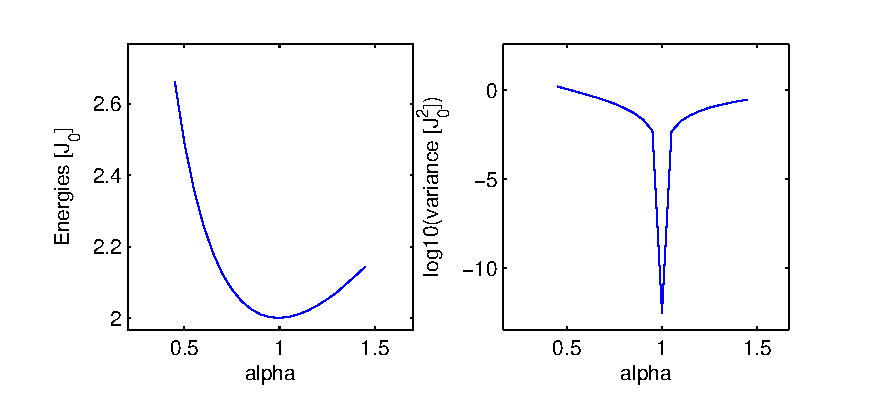
\includegraphics[width=\textwidth]{results/N2_norep.eps}
	\caption{Plot of the values given in table \ref{tab:N2_norep}, the brute force VMC simulation of the two-electron no repulsion or Jastrow factor case. 
	Some of the first values of $\alpha$ has been omitted to make the graph more informative.}
	\label{fig:N2_norep}
\end{figure}

The figure shows exactly what we would expect from the discussion of section \ref{sec:motivation}. 
The energy is always larger than $2$ a.u. and takes this value only when $\alpha = 1$. 
We also see a huge drop in the variance just as we reach $\alpha = 1$ which indicates that this is indeed an eigenstate of the system.
What little is rest of the variance at $\alpha=1$ can be due to numerical errors in the calculation of the laplacians. 
This has in retropspect been verified to be true by using the analytical expression for the local energy. 

Table \ref{tab:N6_N12_norep} shows the result from the $N=6$ and $N=12$ electrons case with no repulsion using the brute force approach with numerical evaluation of the local energy.

\begin{table}[h!]
	\centering 
	\begin{tabular}{l @{}l @{ } l @{ } l @{ } l @{ } l @{ } l}
		\toprule
		\multirow{3}{*}{N=6}$~~\quad ~~$ & $\alpha~~~~$ & $0.9~~~~~~~~~~~~~$ & $0.95~~~~~~~~~~~~~$ & $1~~~~~~~~~~~~~$ & $0.105~~~~~~~~~~~~~$  & $0.11$ \\
		 & $E$(a.u) & 15.0803 & 15.0850 & 15 & 15.0184 & 15.0708\\ 
		 & $\textrm{Variance} ~~$ & 2.49e-1 & 5.89e-2 & 2.56e-13 & 2.36e-2 & 2.05e-1\\ 
		\midrule
		\multirow{3}{*}{N=12} & $\alpha~~~~$ & $0.9~~~~$ & $0.95~~~~$ & $1~~~~$ & $0.105~~~~$  & $0.11$ \\
		& $E$(a.u) & 42.2114 & 42.0497 & 42 & 42.0563 & 42.1937 \\ 
		& $\textrm{Variance} ~~$ & 6.92e-1 & 1.66e-1 & 1.72e-10 & 1.48e-1 & 5.69e-1\\ 
		\bottomrule
	\end{tabular}
	\caption{The results from calculating the expectation value of the local energy and its variance.
			We see that the code works for the $N=6$ and $N=12$ case because we are producing the expected results, $E_6 = 15$ and $E_{12} = 42$ ($\omega = 1.5$). 
			The variance at $\alpha=1$ is so small that we have probably the exact wavefunction.}
	\label{tab:N6_N12_norep}
\end{table}

The table shows that we are able to produce the results we anticipated.
What little there is of variance at $\alpha=1$ is probably due the numerical evaluation of the local energy, which has been confirmed in retrospect by using the analytical expression for the local energy. 
It also shows that the code has implemented the oscillator frequency $\omega$ correctly. 










\subsubsection{Benchmark for the brute force approach, with repulsion and jastrow factor}\label{sec:res_N2_rep}

A plot of the energies and $log_{10}$ of the variances after the investigation is shown in figure \ref{fig:N2_rep}.

\begin{figure}[h!]
	\centering
	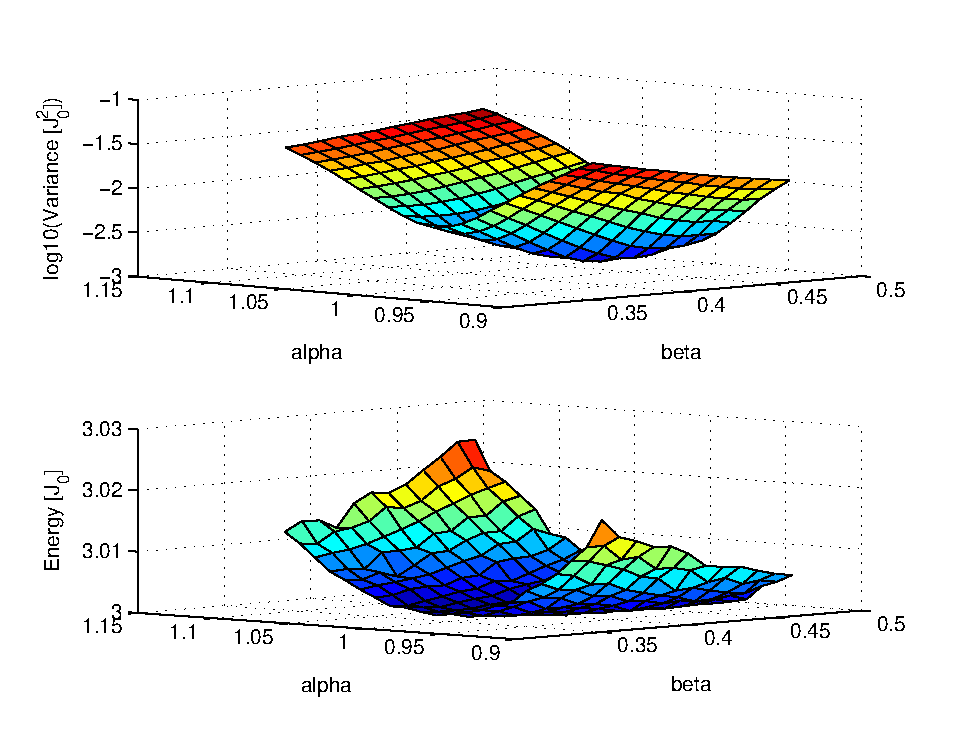
\includegraphics[width=\textwidth]{results/N2_rep.eps}
	\caption{Plot of the expectations of the local energy and $log_{10}$ of variances after the VMC simulations with two electrons, with repulsion and jastrow factor. 
	Each point was based on $10^6$ simulations. 
	The figure gives an overview of how the energies vary as function of $\alpha$ and $\beta$.
	The lowest energy $E= 3.00022$ where $\alpha = 0.98$ and $\beta = 0.42$.}
	\label{fig:N2_rep}
\end{figure}

It is not easy to see from the figure what is the lowest energy, but manipulating the figure in matlab revealed the smallest test state energy, which is given in table \ref{tab:N2_rep}.

\begin{table}[h!]
		\centering 
	\begin{tabular}{l}
		\toprule
		The lowest energy $E=3.00022$ and $\textrm{Variance} = 0.001568$ at $\alpha = 0.98$ and $\beta = 0.42$. \\
		\bottomrule
	\end{tabular}
	\caption{The lowest energy found from the VMC study of the two electron case with repulsion and Jastrow factor.}
	\label{tab:N2_rep}
\end{table}

The lowest energy was also found in the region where the variance was lowest. 
It seems thus that the value obtained in this VMC calculation was very close to the real lowest eigenstate. 
Very close, however, does not mean that we have found \textit{the} eigenstate. 
As we saw in the previous section, when we hit the real eigenstate, the variance dropped rapidly to sizes in order of magnitude $10^{-12}-10^{-13}$ which was not the case here. 



\subsubsection{Comparison of different methods}\label{sec:res_methods_E}

The results from calculation $\langle E \rangle$ for the different method combinations and problem/wave function parameters are shown in table \ref{tab:methods_E}.

\begin{table}[h!]
	\centering
	\begin{tabular}{l @{ } l @{ } l @{ } l @{ } l @{ } l @{ } l  @{ } l  @{ } l  @{ } l }
	\toprule
	  & \multicolumn{3}{c}{Problem and Wavefunction parameters} \\
	 Method parameters $~~~~$ & (2, 1, Jf, 0, 1, Ef) $~$ & (12, 0.5, Jf, 0, 1.5, En) $~$ & (6, 0.82, Jo, 0.22, 3, En)  \\
	\midrule
	(BF, NLE) & 				(2.000, 6e-13)		&		(92.10, 67.54)		&		(54.74, 28.11)			\\
	\shaderow (BF, ALE)	 &		(2.000, 0)			&		(92.18, 161.4)		&		(54.72, 28.19)		\\
	(IS, NLE, NQF) & 			(2.000, 6e-14)		&		(92.15, 66.43)		&		(54.72, 27.33)				 \\
	\shaderow(IS, NLE, AQF) &	(2.000, 1e-13) 		&		(92.06, 54.49)		&		(54.72, 27.32)						\\
	(IS, ALE, NQF) &			(2.000, 0)			&		(92.13, 143.2)		&		(54.76, 27.35)					\\
	\shaderow (IS, ALE, AQF) &	(2.000, 0) 			&		(92.12, 76.24)		&		(54.74, 27.44)	 				\\
	\bottomrule
	\end{tabular}
	\caption{A table of the expectation value and variance (Energy, Variance) of the local energy obatined with different Problem/Wavefunction parameters (N,$\alpha$, Jn/Jf, $\beta$, $\omega$, En/Ef). For explanation of abbreviations, see section \ref{sec:exp_methods_E}.
	For all trials, $10^6$ VMC calculations were performed and for the importance sampling methods, a timestep of $\delta t = 0.1$ was used.}
	\label{tab:methods_E}
\end{table}

These are very strong results. 
Firstly, we have verified the nummerical brute force method against known benchmarks and seen that they are correct,
thus, it seems that the other methods are working properly!
Secondly, the different methods used very different ways to obtain the results. 
That the results are almost the same is a strong indication that all the methods are doing the same thing and working correctly. 















\subsection{Optimizations and differences} \label{sec:res_opt_and_diff}

\subsubsection{Test cases} \label{sec:res_test_cases}

The results from finding the optimal parameters for $\alpha$ and $\beta$ for the different test cases are given in table \ref{tab:test_cases}.

\begin{table}[h!]
	\centering 
	\begin{tabular}{c  c c  c  c  c  c }
	\toprule
	 Test cases: 			& \multicolumn{2}{c}{$\omega=0.01$} & \multicolumn{2}{c}{$\omega=0.10$} & \multicolumn{2}{c}{$\omega=0.28$} \\
	 Optimal parameters  & No Jast. & 	Jast. & 	No Jast. & 	Jast &		No Jast. & 	Jast. \\
	 \midrule
	 $\alpha$& 				0.30 & 		0.91 & 		0.56	&	0.93	&	0.60 & 		0.96 		\\
	 $\beta$ & 				- & 		0.07 & 		-		&	0.18	&	- & 		0.26 	\\
	 \midrule
	 Energy (a.u.) & 		1.03e-1 &	7.40e-2 &	5.25e-1	&	4.41e-1	&	1.14  &		1.02 \\
	 Variance & 			1.12e-2 &	1.48e-5	& 	1.53e-1	&	2.76e-4	&	9.43e-1 & 	7.05e-4 	\\
	\bottomrule
	\toprule
	 Test cases: 			& \multicolumn{2}{c}{$\omega=0.50$} & \multicolumn{2}{c}{$\omega=0.75$} & \multicolumn{2}{c}{$\omega=1$} \\
	 Optimal parameters  & No Jast. & 	Jast. & 	No Jast. & 	Jast. & 	No Jast. & Jast. \\
	 \midrule
	 $\alpha$& 				0.70 & 		0.97 & 		0.74 & 		0.98 	& 	0.72	& 	0.97 	\\
	 $\beta$ & 				- & 		0.32 & 		- & 		0.38 & 		-  		& 	0.42 	\\
	 \midrule
	 Energy (a.u.) & 		1.80 &		1.66 &		2.50  &		2.34 & 		3.15 & 		3.00	\\
	 Variance & 			1.25 &		1.01e-3	& 	1.69 & 		1.35e-3 & 	2.03 & 		2.7e-3 	\\
	 \bottomrule
	\end{tabular}
	\caption{The optimal parameters with and without Jastrow factor (Jast.).
			 Results were produced by calculating the energy for every $\alpha$ and $\beta$ in the interval $[0,1.2]$ with 	a step length of $0.01$ and $10^5$ MC simulation.
			 The estimates with the Jastrow factor seem to be better than those without, though the importance seem to decrease with increasing oscillator frequency $\omega$ (see section \ref{sec:res_jastrow}). }
	\label{tab:test_cases}
\end{table}

The result for $\omega =1$ with jastrow factor is almost in perfect agreement with what was found in section \ref{sec:N2_rep}, even though the method of finding the optimal parameters was different. 
Since only $10^5$ MC simulations were used here, I think this high correspondance is a lucky coincidence, but it does show that the results obtained are reliable, and for the purposes of this section, they are probably good enough. 

Another approach to get these parameters would be to do a simular approach as in section \ref{sec:N2_rep} for each case. 
This proved to be too time-consuming, and an automated approach such as the one used here could be run overnight, which was done here. 
For a further discussion on code efficiency and time constraints, see section \ref{sec:ce_tc}.



\subsubsection{Jastrow factor}\label{sec:res_jastrow}

The relative change in energy (i.e. correlation) due to the Jastrow factor for the test cases is given in table \ref{tab:correlations_jastrow}.

\begin{table}[h!]
	\centering
	\begin{tabular}{ccccccc}
	\toprule
	$\omega$	& 0.01 & 0.10 & 0.28 & 0.50 & 0.75 & 1 \\
	\midrule
	Correlation $C = \frac{E_{NJ} - E_{J}}{E_{NJ}}$ & 0.282 & 0.160 & 0.105 & 0.078 & 0.064 & 0.048 \\
	\bottomrule
	\end{tabular}
	\caption{The correlation introduced by the Jastrow factor for the optimal parameters $\alpha$ and $\beta$ as a function of $\omega$. 
	We see that the correlation factor is less important for high oscillator potentials.
	"NJ" means no Jastrow-factor and "J" means with Jastrow factor.}
	\label{tab:correlations_jastrow}
\end{table}

A plot of the values in table \ref{tab:correlations_jastrow} is given in figure \ref{fig:correlations_jastrow}. 

\begin{figure}[h!]
	\centering 
	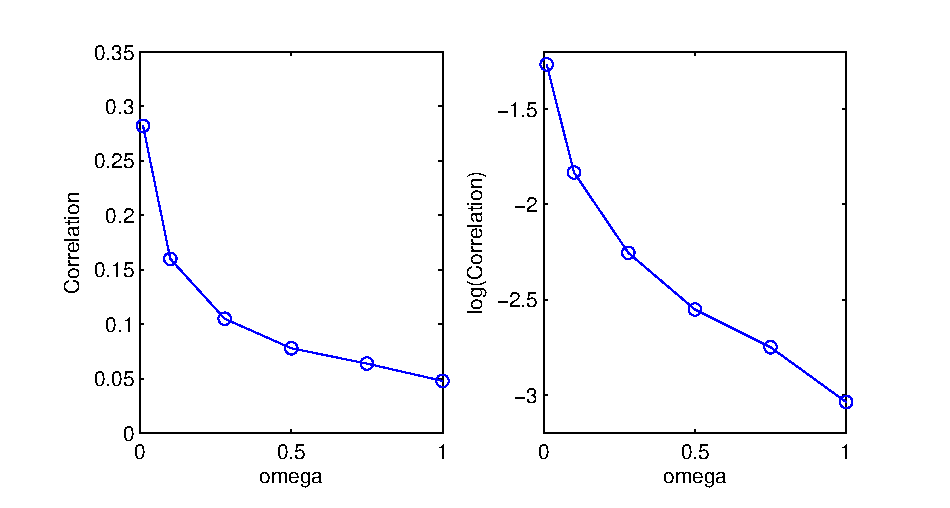
\includegraphics[width=\textwidth]{results/correlations_jastrow.eps}
	\caption{Plot of the correlation introduced by the Jastrow factor for the optimal parameters $\alpha$ and $\beta$ as a function of $\omega$. 
	From the left figure one may suspect a curve of the shape $C = C_0 \exp(-k\omega)$ but the right hand plot of $\textrm{ln}(C)$ against $\omega$ does not look very linear which weakens this hypothesis.}
	\label{fig:correlations_jastrow}
\end{figure}

Our first observation is that the Jastrow factor does indeed better our estimation of the ground state energy. 
We already knew from section \ref{sec:N2_rep} that the including the jastrow factor gave us a very good estimate of the ground state energy when $\omega = 1$, and from table \ref{tab:test_cases}  we see that the ratio between variance and energy estimate is almost constant ($\sim 5 \times 10^{-4}$) in the case with the Jastrow factor as opposed to the case without the Jastrow factor. 

Our second observation from both the table and the figure is that the correlations get smaller as the oscillator frequency increases. 
This is a counter-intuitive result.
Normally one would expect the repulsion between the electrons to be more important the closer together the electrons are.
One can try to explain the phenomenon by looking at another, equivalent expression of the expectation value of the local energy.

\eqs
\langle E_L \rangle = \langle K \rangle + \langle V_{HO} \rangle + \langle V_{ER} \rangle 
\eqf

Where $\langle K \rangle$ is the expection value of the kinetic energy, $\langle V_{HO} \rangle$ that of the harmonic oscillator potential and $\langle V_{ER} \rangle$ that of the electron repulsion potential.
It seems that as $\omega$ increases, all these values increase, but the relative size of $\langle V_{ER} \rangle $ does not increase as much as $\langle V_{HO} \rangle$, so for large $\omega$, the role played by $\langle V_{ER} \rangle$ gets smaller and smaller.

From the left hand plot in the figure, one might suspect that the correlation decreases exponentially as a function of $\omega$. 
To test this, a plot of $\textrm{ln}(C)$ against $\omega$ has been included in the right hand plot. 
If this hypothesis was true, the result should be a straight line, but alas, it is not. 
It is therefore probably some other rule governing the relation between $C$ and $\omega$. 





\subsubsection{Importance sampling} \label{sec:res_importance_sampling}

The results from evaluation $\langle E_L \rangle$ as a function of Monte Carlo simulations and time steps $\delta t$ are given in table \ref{tab:importance_sampling} and figure \ref{fig:importance_sampling}.

\begin{table}[h!]
	\centering 
	\begin{tabular}{l @{ } l @{ } l @{ } l @{ } l @{ } l @{ } l @{ } l @{ } l @{ } l }
	\toprule
	\multicolumn{9}{l}{Energies obtained with the brute force method} \\
	MCS \textbackslash  $\delta t = \quad$ & $10^{-6}~~~$ & $10^{-5}~~~$  & $10^{-4}~~~$  & $10^{-3} ~~~$  & $ 10^{-2} ~~~$ & $ 10^{-1} ~~~$  & $ 1 \qquad $  & $ 10 ~~~~$  & $ 10^{2}$ \\
	\midrule
	$10^3$ & 3.26 &  3.21 & 3.16 & 3.24 &  3.35 &  3.29 & 3.36 &  3.11 &  3.25\\
	\shaderow $10^4$ &  3.21 &   3.22 &    3.22 &   3.27 &  3.25 &  3.26 & 3.24 &   3.22 &  3.26 \\
	$10^5$ & 3.23 &    3.24 &   3.21 &  3.22 &  3.24 &  3.23 & 3.24 &   3.24 &  3.23 \\
	\shaderow $10^6$ & 3.23 &   3.23 &   3.23 &  3.23 &   3.24 &  3.24 & 3.24 &   3.24 &  3.24 \\
	\bottomrule
	\toprule
	\multicolumn{9}{l}{Energies obtained with importance sampling} \\
	MCS \textbackslash  $\delta t = \quad$ & $10^{-6}~~~$ & $10^{-5}~~~$  & $10^{-4}~~~$  & $10^{-3} ~~~$  & $ 10^{-2} ~~~$ & $ 10^{-1} ~~~$  & $ 1 ~~~~$  & $ 10 ~~~~$  & $ 10^{2}$ \\
	\midrule
	$10^3$ & 7.78 &   2.13 &   4.49 &  4.01 &  3.25 &  3.21 &   3.28 &  3.23 &  2.86 \\
	\shaderow $10^4$ &  3.95 &   2.74 &   2.42 &   3.19 &  3.33 &  3.29 &   3.21 &   3.18 &   4.02 \\
	$10^5$ & 2.46 &  3.58 &   3.22 &   3.26 &  3.21 &   3.23 &  3.20 &   3.07 &   5.40 \\
	\shaderow $10^6$ & 3.99 &   3.41 &  3.13 &  3.22 &  3.24 &  3.22 &  3.20 &  4.60 &  2.60 \\
	\bottomrule
	\end{tabular}
	\caption{Energies obtained with the brute force method and the importance sampling method as function of number of  		Monte Carlo simulations (MCS) and time step $\delta t$. 
			Brute force energy estimates do naturally not vary with $\delta t$ since the latter do not play a role in the brute force method. 
			The different energies obtained with the brute force method are thus only repetitions of the same simulation.
			Importance sampling seem to be stable around $\delta t = 10^{-2}$.}
	\label{tab:importance_sampling}
\end{table}


\begin{figure}[h!]
	\centering 
	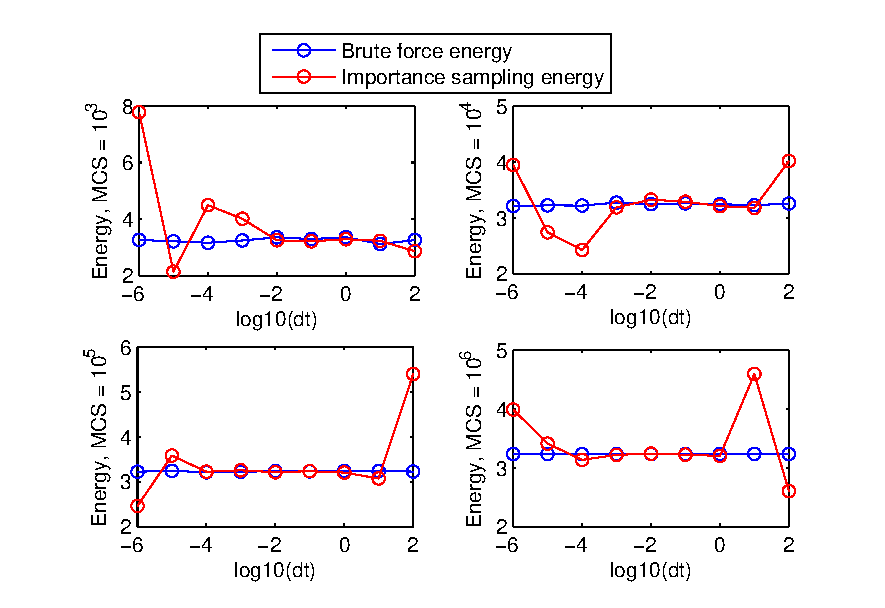
\includegraphics[width=\textwidth]{results/importance_sampling.eps}
	\caption{Plot of the energies evaluated by the brute force method and the metropolis method as a function of number of Monte Carlo simulations (MCS) and time step $\delta t$.}
	\label{fig:importance_sampling}
\end{figure}

We see from the results that the reliability of using importance sampling depends greatly on the time step chosen. 
The results seem to coincide with the brute force method when $\delta t \approx 10^-2 - 10^-2$.
This is natural because if $\delta t$ is too small, the steps in the metropolis algorithm does also become very small. 
It then takes a large number of Monte Carlo simulations for the metropolis walker to move across a representative  selection of points. 
This is illustrated by the figure by noticing that as the number of monte carlo simulations gets larger, a greater range of $\delta t$'s converges to the proper solution. 
When $\delta t$ gets too large, the step length gets too large and we have little control over how the energy estimates will behave. 

The energy estimates by the brute force method does not vary with $\delta t$. 
This is natural because $\delta t$ plays no role in the evaluation of $\langle E_L \rangle$ with the brute force method. 
The different energies obtained for different $\delta t$'s are thus just repetitions of the same measurement, and serve thus only as a illustration of the uncertainty in the evaluation of $\langle E_L \rangle$. 
For the purposes of this project, it seems that the brute force method serves as a stable and reliable method for calculating $\langle E_L \rangle$ with good precision only with a $10^3$ Monte Carlo simulations. 
For more complex problems, it may be that importance sampling, with its foundation in the physical system, attributes to greater precision in producing results, but for the problems discussed here, it seems that it only introduces a new uncertainty in whether the time step $\delta t$ has been chosen correctly. 











\subsubsection{Timely differences between methods} \label{sec:res_timely_diff}

Table \ref{tab:res_times} shows the time used by the different methods for the two different test cases.
A plot of the times used are given in figure \ref{fig:res_times}. 

\begin{table}[h!]
	\centering 
	\begin{tabular}{l @{ } l @{ } l @{ } l @{ } l @{ } l @{ } l @{ } l @{ } l }
	\toprule
	\multicolumn{9}{l}{2 electrons with repulsion and Jastrow factor, $\alpha = 0.77$ and $\beta = 0.22$.} \\
	Method \textbackslash $MCS = ~~~$ & $10^3~~~~~~~$ & $3\times 10^3~~$ & $10^4~~~~~~~$ & $3\times 10^4~~$ & $10^5~~~~~~~$ & $3\times 10^5~~$ & $10^6~~~~$ & $3\times 10^6$ \\
	\midrule
	(BF, NLE) & 1.87e-2 & 4.11e-2 & 1.36e-1 & 2.59e-1 & 7.14e-1 & 2.10 & 6.53 & 19.5 \\
	\shaderow (BF,ALE) & 9.75e-3 & 2.86e-2 & 9.45e-2 & 1.43e-1 & 3.08e-1 & 7.80e-1 & 2.44 & 7.39 \\
	(IS, NLE, NQF) & 1.81e-2 & 5.52e-2 & 1.82e-1 & 5.46e-1 & 1.82 & 5.45 & 18.1 & 54.4 \\
	\shaderow (IS, NLE, AQF) & 1.30e-2 & 3.88e-2 & 1.30e-1 & 3.89e-1 & 1.29 & 3.88 & 12.9 & 38.8 \\
	(IS, ALE, NQF) & 1.12e-2 & 3.22e-2 & 1.08e-1 & 3.19e-1 & 1.06 & 3.18 & 10.7 & 31.9 \\
	\shaderow (IS, ALE, AQF) & 5.30e-3 & 1.59e-2 & 5.28e-2 & 1.59e-1 & 5.30e-1 & 1.59 & 5.30 & 15.9 \\
	\bottomrule
	\toprule
	\multicolumn{9}{l}{6 electrons with repulsion and Jastrow factor, $\alpha = 0.49$ and $\beta = 0.39$.} \\
	Method \textbackslash $MCS = ~~~$ & $10^3~~~~~~~$ & $3\times 10^3~~$ & $10^4~~~~~~~$ & $3\times 10^4~~$ & $10^5~~~~~~~$ & $3\times 10^5~~$ & $10^6~~~~$ & $3\times 10^6$ \\
	\midrule
	(BF, NLE) &  1.44e-1 & 3.85e-1 & 1.25 & 3.06 & 10.0 & 28.4 & 94.3 & 283 \\
	\shaderow (BF,ALE) &  4.75e-2 & 1.47e-1 & 4.89e-1 & 7.79e-1 & 1.86 & 4.80 & 14.8 & 46.2 \\
	(IS, NLE, NQF) & 2.91e-1 & 8.73e-1 & 2.91 & 8.71 & 29.1 & 87.1 & 290 & 870 \\
	\shaderow (IS, NLE, AQF) & 1.91e-1 & 5.71e-1 & 1.90 & 5.70 & 19.0 & 56.9 & 190 & 570 \\
	(IS, ALE, NQF) & 1.40e-1 & 4.20e-1 & 1.40 & 4.19 & 14.0 & 42.0 & 140 & 420 \\
	\shaderow (IS, ALE, AQF) & 3.97e-2 & 1.20e-1 & 3.98e-1 & 1.19 & 4.05 & 11.9 & 39.7 & 120 \\
	\bottomrule
	\end{tabular}
	\caption{Time (in seconds) used by the different methods as a function of Monte Carlo simulations (MCS).
			See section \ref{sec:exp_methods_E} for method abreviations.
			The CPU-time spent using analytical expression is dramatically reduced. }
	\label{tab:res_times}
\end{table}


\begin{figure}[h!]
	\centering 
	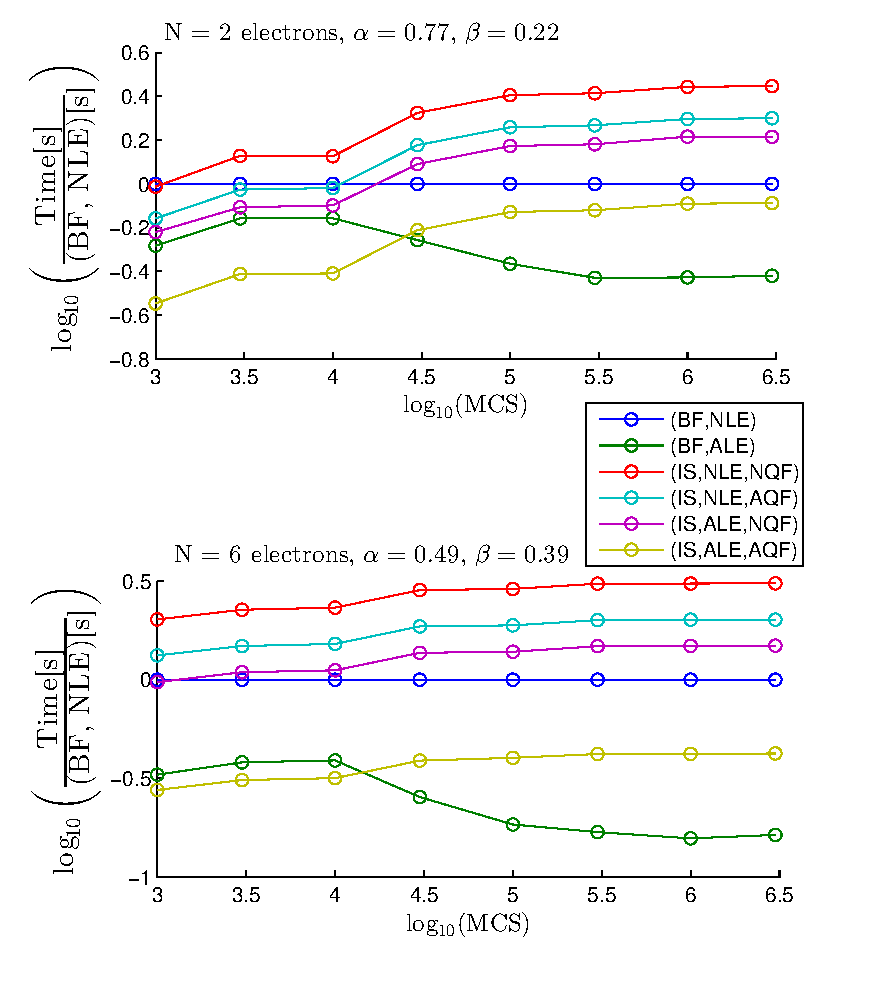
\includegraphics[width=\textwidth]{results/times.eps}
	\caption{$\textrm{log}_{10}$ of the time (in seconds) used by the different methods relative to the brute force, numerical local energy method as a function of $\textrm{log}_{10}$ of Monte Carlo simulations.}
	\label{fig:res_times}
\end{figure}

From the result we see that the relative difference in the time spent by the different methods stabilize after $\sim 10^5$ Monte Carlo simulations. 
After this point, the brute force metropolis algorithm with the analytical expression for the local energy is the most time efficient method, both for $N=2$ and $N=6$. 
To begin with, at $10^3$ Monte Carlo simulations, importance sampling with analytical expressions is the fastest method.
This is because the brute force method needs to run a couple of simulations without sampling to begin with in order to achieve the wanted acceptance rate of $0.5$ whereas the importance sampling method can begin straight away sampling points. 
But as the number of Monte Carlo simulations increase however, this head start gets relatively smaller. 

We also see that whenever analytical expressions is used instead of numerical ones, the efficiency is increased. 
From the figure we see that when using importance sampling, the implementation of the analytical local energy produces a greater increase in efficiency than implementing analytical expressions of the quantum force.
And only when implementing both analytical expressions for the local energy \textit{and} the quantum force is the importance sampling method superior to the brute force, numerical local energy method. 





















\subsubsection{Discussion: code efficiency and time constraints}\label{sec:ce_tc}

The code upon which this project is built has a lot of potential for improvement. 
Lots of the methods developed in this project has been programmed to the point at which the worked, and time constraints have cut short further improvements with regards to code efficacy.
Examples of things that could have improved general code efficacy are things as 

\begin{itemize}
	\item \textbf{Reducing the amount of times a variable is calculated}:
	Although this aspect have been in the back of my mind while programming, I'm sure that a thorough review of the code would reveal a lot of potential. 
	\item \textbf{Avoiding too many divisions}: 
	Divisions in a computer is normally more slow than multiplication\footnote{Source: \href{http://streamcomputing.eu/blog/2012-07-16/how-expensive-is-an-operation-on-a-cpu/}{http://streamcomputing.eu/}}. Replacing recurrent divisions by clever multiplication might have improved code efficiency.
	\item \textbf{Reduce usage of complicated functions such as $\sin$, $\exp$ etc}:
	Although I have put some thought into this while designing the code, there are probably some places where a lot of CPU time could be saved. 
\end{itemize}

There are also things in this specific project that could have improved code efficiency. Examples are

\begin{itemize}
	\item \textbf{More efficient ratio calcuations}:
	In the Metropolis algorithm used in this project, a ratio of the wavefunctions squared was evaluated. 
	But since we only move \textit{one} particle at a time, a lot of the so-called \textit{co-factors} in the Slater determinant cancel\footnote{Page 81, \cite{master}.} and reduces the number of expressions we need to calculate. 
	\item \textbf{Reusage of some expressions}:
	In the calculation of the analytical local energy, the terms needed for the analytical quantum force was also calculated. Implementing this into the code so that if the analytical expression for the local energy was evaluated \textit{and} importance sampling was used with analytical quantum force, the expressions would reused and not calulated twice. 
	There might also be other such examples of expressions which are evaluated multiple times in this code.
	\item \textbf{Better usage of OpenMP parallelization}:
	An interesting question is how much time it takes for OpenMP to communicate between the different threads.
	If this would prove itself a significant issue, then a better implementation of parallelization could have saved some time. 
\end{itemize}

Finally there is the matter of method for finding the optimal parameters $\alpha$ and $\beta$. 
In this project, I used a very brute force method for which I could only spare $10^5$ MC simulations for each energy in order for the process not to take days. 
A better algorithm for finding the optimal $\alpha$ and $\beta$ was not in the scope of this project, but I believe it could seriously improve the efficacy of the process.

But all things considered, I am happy to have paid the price of a slow running code in exchange for having been able to implement lots of different methods for solving the problems discussed in this project. 
Even though the weak efficiency is probably affecting the precision of the result in the next section in a negative manner, the results are still correct within a certain margin of error.
Also, the code is not going anywhere, so if I later want to improve upon it and implement better algorithms for finding $\alpha$ and $\beta$ I am free to do so, even I don't have time to do so before the deadline of this project. 









\subsection{Applications}

\subsubsection{Properties of the approximated wavefunctions} \label{sec:prop_of_app}

The properties of the wavefunctions in this perturbed potential are given in table \ref{tab:interesting_quantitites}. 

\begin{table}[h!]
	\centering 
	\begin{tabular}{l@{ } l@{ } l@{ } l@{ } l@{ } l@{ } l}
		\toprule
		$N=2$ electrons & $\omega = 0.01 \quad $ &  $\omega = 0.10 \quad $ & $\omega =0.28 \quad $  & $\omega = 0.5 \quad $ & $\omega = 0.75 \quad $ & $\omega = 1$ \\
		\midrule
		Energy $\langle H \rangle$  & 	7.40e-2 & 4.41e-1 & 1.02  & 1.66 & 2.34 & 3.00\\
		\shaderow Variance  &	1.09e-5 & 2.74e-4 & 6.86e-4 & 1.03e-3  & 1.32e-3 & 1.78e-3 \\
		Average distance & 	14.7 & 3.36 & 1.76 & 1.24 & 9.62e-1 & 8.17e-1 \\
		\shaderow Potential Energy $\langle V \rangle  \quad $ & 6.43e-2 & 3.5e-1 & 7.71e-1 & 1.22 & 1.67 & 2.12 \\ 
		Kinetic Energy $\langle T \rangle$ &  9.74e-3 & 9.09e-2 & 2.51e-1  & 4.44e-1 & 6.70e-1 & 8.81e-1 \\
		\bottomrule
		\toprule
		$N=6$ electrons & $\omega = 0.01$ &  $\omega = 0.10$ & $\omega =0.28$ & $\omega = 0.5$ & $\omega = 0.75$ & $\omega = 1$ \\
		\midrule
		Optimal $\alpha$ & 0.61 & 0.83 & 0.88 & 0.93 & 0.9 & 0.93 \\
		\shaderow Optimal $\beta$  & 0.10 & 0.22 & 0.33 & 0.38 & 0.5 & 0.57 \\
		Energy $\langle H \rangle$  & 6.99e-1 & 3.57 & 7.62 &  11.8 & 16.1 & 20.2 \\
		\shaderow Variance  & 2.98e-4 & 4.52e-3 & 1.88e-2  & 4.59e-2 & 8.42e-2 & 1.33e-1 \\
		Average distance & 99.1 &	22.9 & 12.1 & 8.56 & 6.70 & 5.57 \\
		\shaderow Potential Energy $\langle V \rangle $ & 6.71e-1 &  3.24 & 6.68 & 10.1 & 13.5 & 16.6 \\ 
		Kinetic Energy $\langle T \rangle$ & 2.76e-2 &  3.30e-1 & 9.56e-1 & 1.74 & 2.6 & 3.62 \\
		\bottomrule
	\end{tabular}
	\caption{Interesting quanttities. 
			The optimal wavefunction parameters used for the $N=2$ electrons case are given in table \ref{tab:test_cases}.}
	\label{tab:interesting_quantitities}
\end{table}

First of all, we notice that the energies obtained here, with $10^7$ Monte Carlo simulations, is the same as the ones obtained in section \ref{sec:res_test_cases} with $10^5$ Monte Carlo simulations to the third digit.
Which is an indication that $10^5$ simulations to find $\alpha$ and $\beta$ was not to little. 

As we might expect, the higher the frequency of the oscillator potential, the closer the electrons are to each other.
This is because the electrons are "squeezed" together by the potential.  
A plot of the average electron distance for both $N=2$ electrons and $N=6$ electrons as a function of $\omega$ is given in figure \ref{fig:AD_electrons}.

\begin{figure}[h!]
	\centering 
	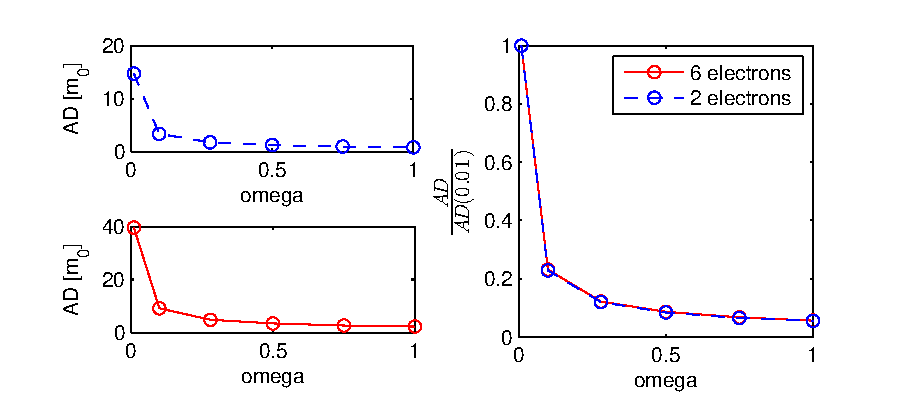
\includegraphics[width=\textwidth]{results/AD.eps}
	\caption{Plot of the average distance (AD) between the electrons for the optimal trial wavefunction for $N=2$ electrons and $N=6$ electrons. 
			The average distance decreases with $\omega$, as expected, when the potential "squeezes" the electrons together.
			The dependancy of AD on $\omega$ is remarkebly similar for $N=2$ electrons and the $N=6$ electrons case.}
	\label{fig:AD_electrons}
\end{figure}

From the figure we see that the 









\subsubsection{The virial theorem }